\documentclass{beamer}
\usepackage{amsmath}
\usepackage{fancybox}
\usepackage{framed}
\usetheme[pageofpages=/,% String used between the current page and the
                         % total page count.
          bullet=circle,% Use circles instead of squares for bullets.
          titleline=true,% Show a line below the frame title.
          alternativetitlepage=true,% Use the fancy title page.
          titlepagelogo=pict/lambang-its-bw-std,% Logo for the first page.
                                % than watermarkheight.
          ]{Torino}
          
% to continu numbering
\newcounter{saveenumi}
\newcommand{\seti}{\setcounter{saveenumi}{\value{enumi}}}
\newcommand{\conti}{\setcounter{enumi}{\value{saveenumi}}}
\resetcounteronoverlays{saveenumi}

% for box
\usepackage{empheq}
\usepackage{graphicx}

\author{Bagus Tris Atmaja\\bagus@ep.its.ac.id}
\title{REVIEW MATEMATIKA SMA}
\institute{Institut Teknologi Sepuluh Nopember}
\date{\today}

\begin{document}

\begin{frame}[t,plain]
\titlepage
\end{frame}

\begin{frame}[t,fragile]{Structure }
\tableofcontents[section]
\end{frame}

\section{1. Pembagian, Perpangkatan dan Akar}
\begin{frame}[t]{Pembagian}
\begin{center}
\fbox{$\cfrac{a}{b}=c$ artinya $ a = b.c $}
\end{center}
\begin{itemize}
    \item Jika $b \neq 0$, maka $\cfrac{0} {b} = 0$, sebab $b.0 = 0$
    \item Jika $a \neq 0$, maka $\cfrac{a} {0}$ tidak didefinisikan. 

    Sebab andaikan $\cfrac{a}{0} = m$ maka $ a = 0.m$, ini tidak ada nilai $m$ yang memenuhi.
    \item Pernyataan $\cfrac{0}{0}=TAK \, TENTU$, sebab andaikan $\cfrac{0}{0} = n$ maka $0=0.n$, Jadi nilai n tidak tunggal.
\end{itemize}
\end{frame}

\begin{frame}[t]{Perpangkatan}
%\begin{columns}
%    \column{.5\textwidth}
        \begin{itemize}
        \item $ a^{m} . a^{n} =a^{m+n} $ \\
        \item $ (ab)^{n} = a^{n}+b^{n} $ \\
%        \end{itemize}
%    \column{.5\textwidth}
%        \begin{itemize}
        \item $ (a^{m})^{n} = a^{mn}$
        \item Jika $a \neq 0$ dan berhingga maka $a^{0}=1$
        \item Jika $a \neq 0$ maka $\cfrac{a^m}{a^n}=a^{m-n}$
        \item Jika $a \neq 0$ maka $ a^{-n}=\cfrac{1}{a^{n}}$
        \end{itemize}
%\end{columns}
\end{frame}

\begin{frame}[t]{Akar}
\begin{itemize}
\item Jika $n$ bilangan bulat positif yang memenuhi $a^n=b$, maka a disebut akar ke $n$ dari $b$. Ditulis  $a=\sqrt[n]{b}$  atau $a=b^\frac{1}{n}$.
\begin{block}{}
\begin{enumerate}
    \item ${\sqrt[n]{a}}^n = a$
    \\
    \hfill \item $\sqrt[n]{\frac{a}{b}}=\frac{\sqrt[n]{a}}{\sqrt[n]{b}}$
    \\
    \hfill \item $\sqrt[n]{ab}=\sqrt[n]{a} . \sqrt[n]{b}$
    \\
    \hfill \item $\sqrt[m]{\sqrt[n]{a}}=\sqrt[mn]{a}$
    \\
\end{enumerate}
\end{block}
\end{itemize}
\end{frame}

\section{2. Persamaan Kuadrat}
\begin{frame}[t,fragile]{Persamaan Kuadrat}
\center \fbox{$ax^2+bx+c=0$, $a \neq 0$ mempunyai akar-akar $x_1$ dan $x_2$}
\newline
\newline
\begin{enumerate}

\item $x_{1,2}=\cfrac{-b \pm \sqrt{b^2-4ac}}{2a}$ atau $x_{1,2}=\cfrac{-b\pm\sqrt{D}}{2a}$ 
\\
\hfill

Dimana $D = b^2 - 4ac$ (diskriminan)
\item Jika $D > 0$ $\rightarrow$ PK mempunyai dua akar berlainan.
\item Jika $D = 0$ $\rightarrow$ PK mempunyai akar real kembar. 
\item Jika $D < 0$ $\rightarrow$ PK tidak punya akar real.
\item $x_1 + x_2 = - \cfrac{b}{a}$; $x_1.x_2=\cfrac{c}{a}$
\end{enumerate}
\end{frame}

\section{3. Fungsi Kuadrat}
\begin{frame}[t,fragile]{Fungsi Kuadrat}
\center \fbox{$y=ax^2+bx+c$; $ a \neq 0$}
\newline
\begin{enumerate}

\item Puncak: $P(- \frac{b}{2a}, - \frac{D}{4a})$
\hfill
\item Jika $a > 0 \rightarrow$ grafik berupa parabola yang membuka ke atas
      $y_{min} = - \frac{D} {4a}$
\item Jika $a < 0 \rightarrow$ grafik berupa parabola yang membuka ke bawah
      $y_{max} = - \frac{D}{4a}$
\item Jika $D > 0 \rightarrow$ y memotong sumbu x di dua titik yang berlainan
\item Jika $D = 0 \rightarrow$ y menyinggung sumbu x
\item Jika $D < 0 \rightarrow$ y tidak memotong sumbu x
\item Jika $D \leqq 0 \rightarrow$ y tidak memotong sumbu x di dua titik
    \seti
\end{enumerate}
\end{frame}


\begin{frame}[t] {Fungsi Kuadrat (Cont'd)}
\begin{enumerate}
\conti
\item Fungsi Kuadrat disebut \emph{definit positif} jika grafik seluruhnya berada 
      di atas sb x; Syaratnya: \hspace{0.05in}           (1) $a > 0$
                            
      \hspace{1.62in}          (2) $D <0$
\hfill
\item Fungsi Kuadrat disebut \emph{definit negatif} jika grafik seluruhnya berada 
      di bawah sb x; Syaratnya: \hspace{0.05in}           (1) $a < 0$
                            
      \hspace{1.76in}          (2) $D > 0$
\end{enumerate}
\end {frame}

\section{4. Logaritma}
\begin{frame}[t,fragile]{Logaritma}
\fbox{\parbox{\dimexpr\linewidth-2\fboxsep-2\fboxrule}{\centering 
        $^{a}\log{b}=c$ artinya: $a^c=b$\\
        syarat: $b > 0$, $a > 0$, $a \neq a$.\\
        $a$ disebut bilangan pokok.}}
\vskip12pt
Sifat-sifat:
\begin{columns}
\column{.5\textwidth}
\begin{enumerate}
    \item $a^{^{a}\log{b}}=b$
    \item $^{a}\log{a}=1$
    \item $^{P}\log{a}+^{P}\log{b}=^{P}\log{ab}$
    \item $^{P}\log{a}-^{P}\log{b}=^{P}\log{\frac{a}{b}}$
    \item $^{P}\log{a^n} = n ^{a}\log{a}$
    \item $^{a}\log{a^n} = n$
    \item $^{a}\log{1} = 0$
    \seti
\end{enumerate}
\column{.5\textwidth}
\begin{enumerate}
    \conti
    \item ${^{a}\log{b}}=\frac{^{P}\log{a}}{^{P}\log{b}}$
    \item $^{a}\log{b}^{b}\log{c}=^{a}\log{c}$
    \item $^{a}\log{b}^{b}\log{c}=1$
    \item $^{a}\log{\sqrt[n]{b}=\frac{1}{n}^{a}\log{b}}$
    \item $^{a}\log{b} = \frac{1} {^{b}\log{a}}$
    \item $^{a}\log{\frac{1}{b}} = - ^{a}\log{b}$

\end{enumerate}
\end{columns}
\end{frame}

\begin{frame}[t,fragile]{Bilangan "e"}
Definisi:

\begin{center}
\fbox{$\underset{n\rightarrow\infty}{\lim}{1+\frac{1}{n}^n}=e=2.7182818$}
\end{center}
\begin{itemize}
\item Log dengan bilangan pokok e disebut logaritma natural
$^{a}\log x = \ln x$ dibaca lon x; $\ln e=1; \ln 1 = 0$
\item Hubungan $\log$ dengan $\ln$:
\vskip12pt
\fbox{$\log x = 0.4345 \ln x; \ln x= 2.3028 \log x$}
\end{itemize}
\end{frame}

\section{5. Goniometri}
\begin{frame}[t,fragile]{Goniometri}
\begin{columns}
\column{.4\textwidth}
\includegraphics[width=1.7in]{pict/segitiga}
\column{.3\textwidth}
$\sin{\alpha}=\cfrac{BC}{AC}$
\\
$\cot{\alpha}=\cfrac{AB}{BC}$
\\
$\tan{\alpha}=\cfrac{\sin{\alpha}}{\cos{\alpha}}$
\\
$\sec{\alpha}=\cfrac{1}{\cos{\alpha}}$
\\
$\cos{\alpha}=\cfrac{AB}{AC}$
\\
$\sec{\alpha}=\cfrac{AC}{AB}$
\column{.3\textwidth}
$\cot{\alpha}=\cfrac{\cos{\alpha}}{\sin{\alpha}}$
\\
$\csc{\alpha}=\cfrac{1}{\sin{\alpha}}$
\\
$\tan{\alpha}=\cfrac{BC}{AB}$
\\
$\csc{\alpha}=\cfrac{AC}{BC}$
\\
$\tan{\alpha}=\cfrac{1}{\cot{\alpha}}$
\\
\end{columns}
\end{frame}

\section{6. Segitiga Pascal}
\begin{frame}[t,fragile]{Segitiga Pascal}
\vspace{20pt}
\begin{columns}
\column{.35\textwidth}
\begin{center}
    \includegraphics[width=1.5in]{pict/pascal}
\end{center}

\column{.65\textwidth}
$(a+b)^0=1$
\\
$(a+b)^1=a+b$
\\
$(a+b)^2=a^2+2ab+b^2$
\\
$(a+b)^3=a^3+3a^2b+3ab^2+b^3$
\\
$(a+b)^4=a^4+4a^3b+6a^2b^2+4ab^3+b^4$
\\
$(a+b)^5=a^5+5a^4b+10a^4b^2+10a^2b^3+5ab^4+b^5$
\\
dan seterusnya...
\end{columns}

\end{frame}

%\watermarkon

\section{7. Satuan Imaginer dan Perkalian Istimewa}
\begin{frame}[t, fragile]{Satuan Imaginer}
\begin{center} \fbox {$i=\sqrt{-1};\, i^2=-1$}
\vskip12pt
\begin{itemize}
\item Bilangak kompleks: $z=a+bi$; $a=$ bagian real dari bilangan komplek z,
                                    $b=$ bagian imaginer dari z.
\item Ingat bahwa: $\sqrt{ab}=\sqrt{a}.\sqrt{b}$, sehingga: $\sqrt{-3}=\sqrt{-1}.\sqrt{3}=i\sqrt{3}$
\\
$\sqrt{-9}=\sqrt{-1}.\sqrt{9}=i\sqrt{9}=i.3=3i$
\item Akar-akar dari PK: $x^2+x+1=0$ adalah:
\vskip10pt
$x_{1,2}=\cfrac{-1\pm\sqrt{1^2-4(1)}}{2}=\cfrac{-1\pm\sqrt{-3}}{2}=\cfrac{-1\pm\sqrt{-3}{i}}{2}$
$x_{1}=\cfrac{-1}{2}+\cfrac{\sqrt{3}{i}}{2}$
\hskip40pt
$x_{2}=\cfrac{-1}{2}-\cfrac{\sqrt{3}{i}}{2}$
\end{itemize}
\end{center}
\end{frame}

\section{8. Geometri Analitik Datar }
\begin{frame}[t, fragile]{Geometri Analitik Dasar}
\begin{enumerate}
\item Garis lurus
\item Lingkaran
\item Parabola
\item Ellips
\item Hyperbola
\end{enumerate}
\end{frame}

\begin{frame}[t, fragile]{Garis Lurus}
\begin{enumerate}
\item Jarak $A(x_A, y_A)$ ke $B(x_B,y_B)$ adalah $AB=\sqrt{(x_B-x_A)^2+(y_B-y_A)^2}$
\item Persamaan explisit garis lurus $y=mx+n$\\
      (m= Koefisien arah/bilangan arah)
\item Persamaan impisit gari lurus $ax+by+c=0$ dengan bilangan arah $m=-\frac{a}{b}$
\item Jarak dari $A(x_A, y_A)$ ke garis $ax+by+c=0$ adalah\\
      $d=\Bigl\vert\cfrac{ax_{A}+by_{A}+c}{\sqrt{a^2+b^2}}\Bigr\vert$
\item Persamaan garis lurus melalui  2 titik  $A(x_A, y_A)$ ke $B(x_B,y_B)$ \\
      $\cfrac{y-y_A}{y_B-y_A}=\cfrac{x-x_A}{x_B-x_A}$
\end{enumerate}
\end{frame}


\begin{frame}[t, fragile]{Garis Lurus(Cont'd)}
Garis lurus $g: ax+by+c=0$ dengan bilangan arah m1,\\
Garis lurus $h: px+qy+r=0$ dengan bilangan arah m2;\\
maka supaya\\
\hskip40pt $g$ // $h$, syaratnya: $m_1=m_2$\\
\hskip40pt $g\perp  h$, syaratnya: $m_1.m_2=-1$\\
\hskip40pt $g$ memotong $h$, syaratnya: $m_1\neq m_2$\\
\hskip40pt $g$ berimpit dengan $h$, syaratnya: $\cfrac{a}{p}=\cfrac{b}{q}=\cfrac{c}{r}$

\end{frame}

\begin{frame}[t, fragile]{Lingkaran}
\begin{enumerate}
\item Persamaan lingkaran pusat $0(0,0)$, jari-jarinya $a$ adalah : $x^2+y^2=a^2$
\item Persamaan lingkaran pusat $P(a,b)$, jari-jarinya $r$ adalah \\
$(x-a)^2+(y-b)^2=r^2$
\item Lingkaran: $x^2+y^2+Ax+By+C=0$ mempunyai\\
      Pusat di $P(-\frac{1}{2} A, -\frac{1}{2} B)$; jari-jari $r=\sqrt{\frac{1}{4} A^2 + \frac{1}{4} B^2 -C}$
\begin{exampleblock}{Contoh}
Lingkaran: $x^2+y^2-2x-4y+1=0$ mempunyai titik pusat \\ 
di $P(1,2)$ dengan jari-jari $r=\sqrt{\frac{1}{4} {-2}^2 + \frac{1}{4} {-4}^2 -1}=2$
\end{exampleblock}
\end{enumerate}
\end{frame}

\begin{frame}[t, fragile]{Parabola}
%\begin{enumerate}
\underline{Parabola}: Tempat kedudukan titik-titik yang berjarak sama terhadap sebuah titik dan sebuah garis yang tertentu.
      \\ 
      Titik-titik itu disebut \underline{Fokus}; garis itu disebut \underline{Direktrix}.
\vskip10pt
\begin{columns}
\column{.55\textwidth}
\includegraphics[width=2.5in]{pict/parabola}
\column{.45\textwidth}
Ambil SR=sb x; SF=p dan
\newline
OS = OF = $\frac{1}{2} p$
\\
F$(\frac{1}{2}p,0)$ fokus; P(x,y) pada parabola.
\\Pada $\Delta$ siku-siku PFR:
\\$PF^2=PR^2+FR^2$
\\$(x+\frac{1}{2}p)^2=y^2+(x-\frac{1}{2}p)^2$
\\$x^2+px+\frac{1}{4}p^2=y^2+x^2-px+\frac{1}{4}p^2$
\end{columns}
\end{frame}

\begin{frame}[t, fragile]{Parabola(Cont'd)}
\begin{center}
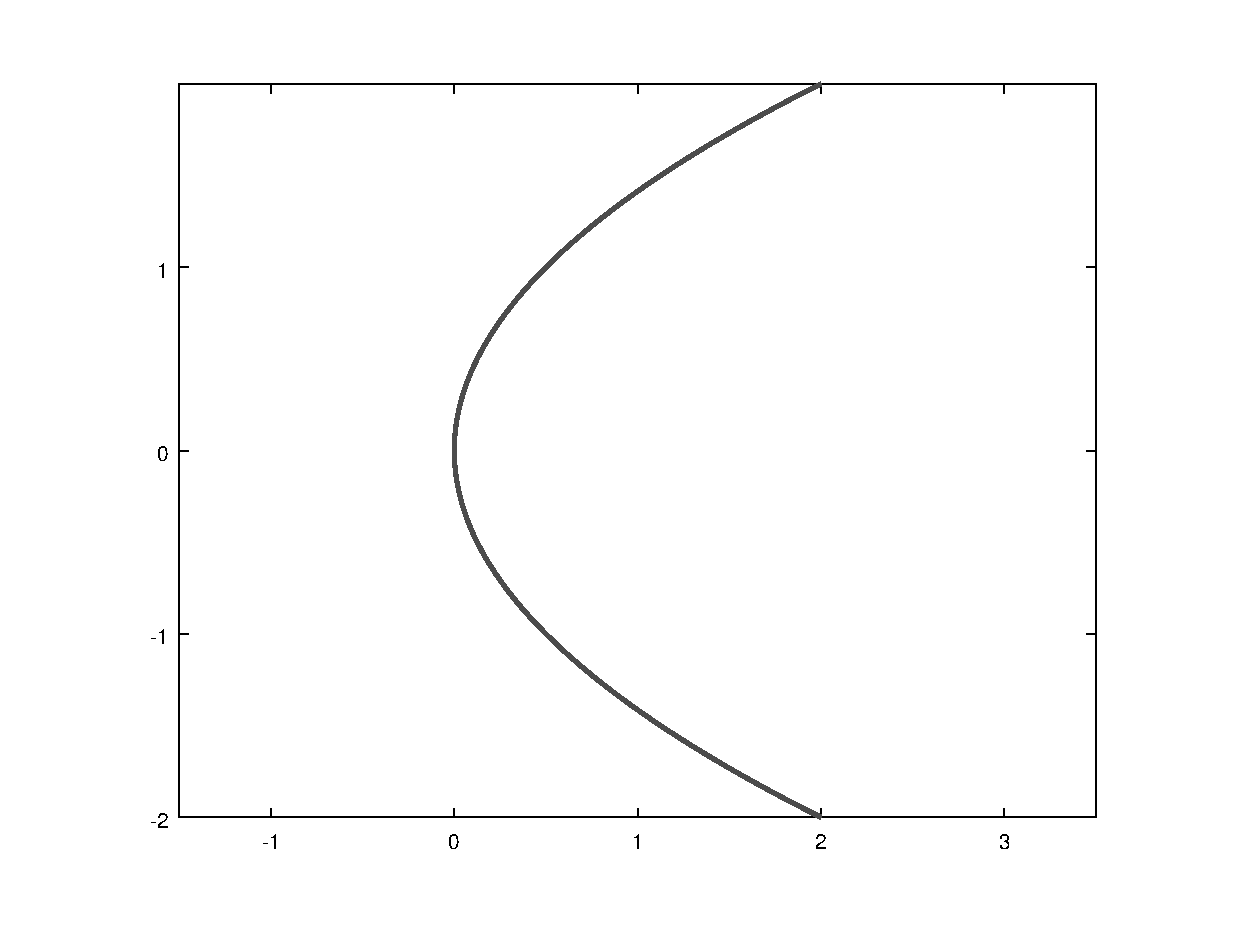
\includegraphics[width=2.3in]{pict/parabola2}
\\
\fbox {$y^2=2px$} p = parameter parabola
\end{center}
Jika puncak parabola (a, b) dan sb. simetri tetap $//$ sb. x, maka persamaan parabolanya:
\begin{center}
{$(y-b)^2 = 2p (x-a)$}
\end{center}
\end{frame}

\begin{frame}[t, fragile]{Ellips}
\underline{Ellips}: Tempat kedudukan titik-titik yang jumlah jaraknya terhadap 2 titik tertentu tetap nilainya.
\begin{columns}
\column{.55\textwidth}
\includegraphics[width=2.5in]{pict/ellips0}
\column{.45\textwidth}
Fokus: F(-c,0) dan G(c,0)
\\
P(x,y) pada ellips maka:\\
PF + PG = 2a (tetap) \\
Kedua titika A dan B memenuhi sebab \\
jika AF = GB = a - c, maka:\\
AF+AG=BF+BG\\
\hskip36pt=(a-c)+(a+c)=2a
\end{columns}
\vskip10pt
$PF=\sqrt{(x+c)^2+y^2}$ dan $PG=\sqrt{(x-c)^2+y^2}$
\\
$PF+PG=2a \rightarrow (a^2-c^2)x^2+a^2+y^2=a^2(a^2-c^2)$
\end{frame}

\begin{frame}[t, fragile]{Ellips(Cont'd)}
Misalkan: $a^2-c^2=b^2$ \\
maka persamaan ellips:
\fbox{$\cfrac{x^2}{z^2}+\cfrac{y^2}{b^2}=1$}  \hskip10pt 2a = Sb. panjang\\
                                             \hskip189pt 2b = Sb. pendek \\
Jika pusat ellips ($\alpha,\beta$) dan sumbu-sumbu simetri tetap $//$ sb. x dan sb. y, maka persamaan ellipsnya:\\
\begin{center}
$\cfrac{(x-\alpha)^2}{a^2}+\cfrac{(y-\beta)^2}{b^2} = 1$
\end{center}
\end{frame}

\begin{frame}[t, fragile]{Hyperbola}
\underline{Hyperbola} ialah tempat kedudukan titik-titik yang selisih jaraknya terhadap dua titik tertentu tetap nilainya.
\begin{columns}
\column{.55\textwidth}
\includegraphics[width=2.5in]{pict/hyperbol1}
\column{.45\textwidth}
Fokus: $F(-c,0)$ dan $G(c,0)$ \\
$AF=BG=c - a $\\
$AG-AF= BF - BG $\\
\hskip47pt$= (c+a) - (c-a)$\\ 
\hskip47pt$= 2a$ \\
P(x,y) pada hyperbola \\
$PF = \sqrt{(x+y)^2 + y^2}$ \\
$PG =\sqrt{x-c)^2+y^2}$\\
\end{columns}
\end{frame}

\begin{frame}[t, fragile]{Hyperbola(Cont'd)}
$PF - PG=2a \rightarrow (c^2 - a^2)x^2-a^2-y^2=a^2(c^2-a^2)$\\
Misalkan: $c^2-a^2 = b^2$\\ 
\vskip5pt
Maka persamaan hyperbola: \fbox{$\cfrac{x^2}{z}^2-\cfrac{y^2}{b^2} = 1$}\\
\vskip5pt
Jika pusat hyperbola ($\alpha, \beta$) dan sumbu-sumbu simetri tetap $//$ sumbu x dan sumbu y; maka persamaan parabolanya:\\
\begin{center}
$\cfrac{(x-\alpha)^2}{a^2} - \cfrac{y^2}{b^2} = 1$\\
\end{center}
Jika a = b; disebut hyperbola ORTHOGONAL (siku-siku).

\end{frame}

\section{9. Fungsi, Nilai mutlak bilangan real, notasi fakulteit dan radian}
\begin{frame}[t,fragile]{Fungsi}
\begin{itemize}
\item Definisi:\\
Variabel y disebut fungsi dari variabel x jika dapat ditentukan hubungan anatara x dan y sedemikian hingga untuk setiap nilai x (yang mungkin diberikan) menentukan secara tunggal nilai y.\\
\vskip5pt
\begin{center} \fbox{$ y = f(x)$}\\
\end{center}
\item $ y \rightarrow $ variabel tak bebas \\
\item $ x \rightarrow $ variabel bebas 
\end{itemize}
\end{frame}

\begin{frame}[t,fragile]{Nilai Mutlak dari bilangan real}
\begin{itemize}
\item Definisi:\\
\hskip20pt $\left| x \right| = \begin{cases} x, \, jika \, x \geq 0 &\\ \\
                -x, \, jika \, x < 0
                \end{cases}$
\begin{exampleblock}{Contoh:}
$\vert 6 \vert = 6$; sebab $6 >0 $\\
$\vert -5 \vert = -(-5)$; sebab $5 \geq 0$
\end{exampleblock}
\end{itemize}
\end{frame}

\begin{frame}[t,fragile]{Notasi Faktorial / Fakulteit}
Definisi: \\
\hskip50pt \fbox{$ n! = 1 . 2 . 3 . 4 ...(n-1).n$}
\begin{exampleblock}{Contoh:}
\begin{enumerate}
\item $1! = 1$;
\item $3! = 3 . 2 .1=6$
\item $0! = 1 (khusus)$
\end{enumerate}
\end{exampleblock}
\end{frame}

\begin{frame}[t,fragile]{Radian}
\begin{columns}
\column{0.4\textwidth}
\includegraphics[width=1.5in]{pict/radian1}
\column{0.6\textwidth}
\begin{itemize}
\item Lingkaran satuan, jari-jari = 1
\item $\cap \, AB = 1 \longrightarrow  \angle AOB = 1$ radian
\item $2 \pi rad = 360^o,  \hskip10pt \frac{1}{3} \pi rad= 60^o$ 
\item $\pi rad = 180^o, \hskip15pt \frac{1}{4} \pi rad= 45^o$ 
\item $\frac{1}{2} \pi rad = 90 ^o, \hskip15pt \frac{1}{6} \pi rad= 30^o$ 
\end{itemize}
\end{columns}
\vskip10pt
\begin{exampleblock}{Contoh:}
1 radian = $\cfrac{360}{2\pi} = \cfrac{360^o}{2(3.14159)}=57^o:$ 7': 45"
\end{exampleblock}
\end{frame}

\end{document}
